\usetikzlibrary{calc}
\usetikzlibrary{intersections}
\usetikzlibrary{angles}
\usetikzlibrary{quotes}

\chapter{Введение}
\noindent\indent Идея создания солнечных парусов возникла ещё в начале XX в.
С того момента, как Максвелл теоретически обосновал, что излучение может создавать давление,
ученые задумались о том, как использовать давление солнца как движущую силу.\par
    В 1924 Константином Циолковским и Фридрихом Цандером впервые был предложен концепт
использования такой конструкции, как солнечный парус, что позволяет использовать
такое явление, как солнечное давление на качественно новом уровне [1].\par
    В 1974 эффект солнечного давления был впервые продемонстрирован на движении межпланетного
космического аппарата Маринер 10 [2]. На солнечные панели Маринера 10 под различными углами к солнцу
действовало различное солнечное давление, что влияло на вращательное движение аппарата.\par
    В конце 70-хх годов в NASA Jet Propulsion Laboratory (JPL) активно стали изучать
возможность использования технологии солнечного паруса для подхода космических аппаратов
вблизи кометы Галлея во время её попадания в 1986 в область Солнечной системы [3].\par
    Ввиду больших затрат энергии для этой миссии, идея использования солнечного паруса
и энергии солнечного давления в целом выглядела весьма перспективной. Однако, в то
время разработки с использованием ионных двигателей были доработаны и составляли
большую конкуренцию солнечному парусу. В сентябре 1977 года в NASA отдали
предпочтение проекту на ионном двигателе, хотя позже и этот проект был свёрнут
из-за недостатка финансирования.\par
    Несмотря на то, что миссия к комете Галлея была свёрнута NASA, разработки солнечного паруса
породили значимый интерес к этой идее и в последнее время NASA, и ESA (European Space Agency)
инициировали программы для создания мало-затратных, но грузоподъёмных кораблей
для планетарных и космических научных миссий. Программа NASA «New Millenium» и
программа ESA SMART опробуют новые технологии для демонстрации возможностей таких
лёгких высокопроизводительных кораблей [4].\par
    В настоящее время некоторые современные концепции солнечного паруса стали меньше
в размерах. Это уменьшение масштаба упрощает производство, упаковку и
развёртывание солнечного паруса. Не нужно больше рассматривать космический
парус как огромную неудобную конструкцию, подлежащую разработке в далёком будущем.
Конструирование, нужное для паруса, приблизилось к реальным масштабам, придавая
большую убедительность идее его использования.\par
    В данный момент на площадке Центра Проектной Деятельности Дальневосточного
федерального университета, было решено спроектировать и создать космический аппарат
на базе спутника <<CubeSat>> с использованием солнечного паруса на борту
с последующим участием в состязаниях <<NTI Sputnik challenge>>.\par
    В рамках данного проекта мною был реализован алгоритм подбора оптимальных
угловых значений ориентации спутника с целью увода спутника на более высокую орбиту
Земли, а также реализована модель движения аппарата по орбите Земли под действием
внешних возмущающих сил.
% \newpage
\chapter{Термины, определения, обозначения и сокращения}
\begin{itemize}
    \item Апогей -- наиболее удаленная от одного из фокусов точка орбиты
    \item Аргумент перигея ($\omega$) -- угловое расстояние от линии узлов в плоскости
    орбиты до направления на перигей орбиты
    \item Аргумент широты ($u$) -- угол, отсчитываемый в плоскости орбиты от линии
    узлов до текущего радиус-вектора орбиты
    \item Восходящий узел -- точка на небесной сфере, в которой спутник пересекает
    экватор в своем движении из южного полушария в северное
    \item Долгота восходящего узла ($\Omega$) -- угол между направлениями на точку весеннего
    равноденствия и на восходящий узел
    \item КА -- космический аппарат
    \item Линия узлов -- линия пересечения плоскостей орбиты и экватора
    \item Нисходящий узел -- узел, противоположный восходящему
    \item Наклонение ($i$) -- угол между экваториальной плоскостью и плоскостью орбиты
    \item ОСК -- опорная система координат
    \item Перигей -- ближайшая к одному из фокусов точка орбиты
    \item ССК -- связанная система координат
    \item Узел орбиты -- следы линии узлов на небесной сфере
\end{itemize}
\newpage
% \section{Неформальная постановка задачи}
% \noindent\indent Реализация математической модели управления КА в рамках данной
% работы включает в себя следующие основные задачи:
% \begin{enumerate}[label=\arabic*.]
%   \item Разработка модуля по расчету результирующих сил и моментов, действующих
%   на солнечный парус
%   \item Реализация алгоритма поиска оптимального управления парусом
%   % \item Интеграция разработанных решений с приложением <<Sputnix Satellite Simulator>>
% \end{enumerate}
\chapter{Описание условий моделирования процесса изменения положения и ориентации
спутникового аппарата}
\section{Уравнения движения}
\noindent\indent Введем следующие системы координат:\par
\noindent $OXYZ$ -- не вращающаяся система координат: ось $OZ$ направлена
перпендикулярно плоскости эклиптики, $OX$ -- направлена в точку весеннего
равноденствия, а $OY$ дополняет эту систему до правой ортогональной системы
координат, начало координат -- центр масс спутника;\par
\noindent $OX_1X_2X_3$ -- опорная система координат (ОСК). В данной работе
этой системой является орбитальная система координат: ось $OX_1$ направлена вдоль
радиус-вектора, направленного к центру масс спутника от барицентра орбиты его движения
 в поле тяготения Земли, $OX_2$ -- по касательной к траектории орбиты в сторону
движения аппарата, $OX_3$ -- дополняет систему до правой ортонормированной системы
координат, -- направлен перпендикулярно к плоскости орбиты;\par
\noindent $Ox_1x_2x_3$ -- связанная система координат (ССК), оси которой являются
главными центральными осями инерции аппарата.\par
    Связь между системами координат $Ox_1x_2x_3$ и $OX_1X_2X_3$ задается двумя
способами: набором углов $\alpha$, $\beta$, $\gamma$ (рисунок \ref{fig:KrilovAngles})
и матрицей направляющих косинусов $A$.\par
    Переход от ОСК к ССК происходит с помощью трех последовательных поворотов
(рисунок \ref{fig:KrilovAngles}). Первый поворот осуществляется относительно оси $OX_2$
на угол $\alpha$, второй -- вокруг оси $Ox_3'$ (образованной после первого поворота
осью $OX_3$) на угол $\beta$, третий -- вокруг оси $Ox_1$ на угол $\gamma$.
\begin{figure}[h]
  \centering
  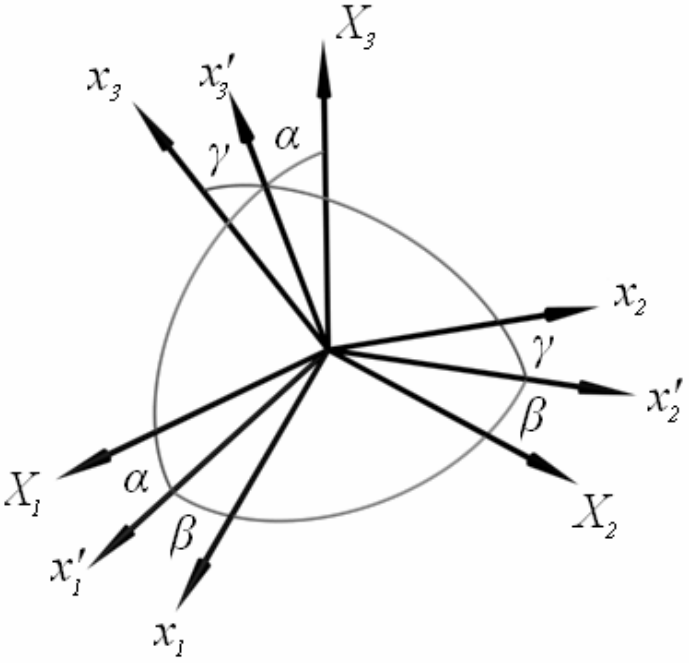
\includegraphics[width=0.4\textwidth]{PlaneAngles}
  \caption{Самолетные углы}
  \label{fig:KrilovAngles}
\end{figure}\par
    Матрица направляющих косинусов через углы Эйлера запишется в виде
\begin{equation}
    A = \begin{bmatrix}
        \cos\alpha\cos\beta & \sin\beta & -\sin\alpha\cos\beta\\
        -\cos\alpha\sin\beta\cos\gamma & \cos\beta\cos\gamma & \sin\alpha\sin\beta\cos\gamma + \cos\alpha\sin\gamma \\
        \cos\alpha\sin\beta\sin\gamma + \sin\alpha\cos\gamma & -\cos\beta\sin\gamma & -\sin\alpha\sin\beta\sin\gamma + \cos\alpha\cos\gamma
    \end{bmatrix}
\end{equation}
Матрица описывает переход из системы координат $OX_1X_2X_3$ в связанную систему
координат $Ox_1x_2x_3$.\par
\noindent\indent Для описания модели изменения ориентации аппарата, используется
закон изменения кинетического момента (динамические уравнения Эйлера):
\begin{equation}\label{eq:EulerDynamic}
    \dot{\vec{K}} + \vec{\omega}_{\text{абс}} \times \vec{K} = \vec{M}_{\text{вш}} + \vec{M}_{\text{упр}},
\end{equation}
и кинематические уравнения:
\begin{equation}\label{eq:EulerKinematic}
    \dot{A} = WA,
\end{equation}
или
\begin{equation}
    \begin{aligned}
        & \dot{\alpha} = \frac{1}{\cos\beta}(\omega_1\cos\gamma - \omega_3\sin\gamma), \\
        & \dot{\beta} = \omega_2\sin\gamma + \omega_3\cos\gamma, \\
        & \dot{\gamma} = \omega_1 - \tg\beta(\omega_2\cos\gamma - \omega_3\sin\gamma),
    \end{aligned}
\end{equation}\par
где $\vec{K} = J\vec{\omega}_{\text{абс}}$ -- кинетический момент аппарата;

$\vec{\omega}_{\text{абс}} = \vec{\omega}_{\text{отн}} + A\vec{\omega}_0$ -- вектор
абсолютной угловой скорости;

$J$ -- тензор инерции тела; $\vec{M}_{\text{вш}}$ -- момент внешних сил;

$\vec{M}_{\text{упр}}$ -- управляющий момент;

$\vec{\omega}_{\text{отн}} = (\vec{\omega}_1\,\, \vec{\omega}_2\,\, \vec{\omega}_3)^T$ --
вектор угловой скорости движения системы $Ox_1x_2x_3$ относительно $OX_1X_2X_3$,
записанный в осях системы $Ox_1x_2x_3$;

$\vec{\omega}_0$ -- абсолютная угловая скорость системы координат $OX_1X_2X_3$,
матрица $W$ имеет вид:
\begin{equation}
    W = \begin{bmatrix}
        0 & \omega_3 & -\omega_2 \\
        -\omega_3 & 0 & \omega_1 \\
        \omega_2 & -\omega_1 & 0
    \end{bmatrix}.
\end{equation}
%
\section{Невозмущенное движение. Кеплеровы элементы орбиты}
\noindent\indent Движение спутника осуществляется в поле тяготения Земли. Основной силой,
действующей на небесное тело является сила всемирного тяготения: две материальные точки,
обладающие массами $m$ и $M$, тяготеют друг к другу с силой
\begin{equation} \label{eq:GForce}
  \vec{F} = G\frac{mM}{r^2},
\end{equation}\par
    где $r$ -- расстояние между центрами тел;\par
    $G$ -- универсальная гравитационная постоянная
($G = 6.67\cdot10^{-8}\text{см}^3/г\cdot\text{сек}^2$).\par
    Если рассматривать движение одного из тел (спутника) с массой $m$ относительно
другой (Земли) с массой $M$, считая, что можно пренебречь всеми силами, кроме силы
(\ref{eq:GForce}), то дифференциальные уравнения движения примут вид:
\begin{equation}
  \begin{aligned}
    &\ddot{x} + \frac{\mu x}{r^3} = 0, \\
    &\ddot{y} + \frac{\mu y}{r^3} = 0, \\
    &\ddot{z} + \frac{\mu z}{r^3} = 0,
  \end{aligned}
\end{equation}\par
    где $\mu = GM$, $x$, $y$, $z$ -- координаты точки (спутника) с массой $m$ в
поступательно перемещающейся системе координат с началом в точке (центре Земли)
с массой $M$;\par
    $r = \sqrt{x^2 + y^2 + z^2}$.\par
В самом деле, здесь пренебрегаются <<посторонние>> силы, действующие на точку c
массой $m$. Но эти силы действуют, и с их учетом уравнения
\begin{equation} \label{eq:GAccelerationModify}
  \begin{aligned}
    &\ddot{x} + \frac{\mu x}{r^3} = a_x, \\
    &\ddot{y} + \frac{\mu y}{r^3} = a_y, \\
    &\ddot{z} + \frac{\mu z}{r^3} = a_z,
  \end{aligned}
\end{equation}\par
    где $a_x$, $a_y$, $a_z$ -- компоненты добавочных ускорений.\par
Уравнения (\ref{eq:GAccelerationModify}), вообще говоря, уже не интегрируются.\par
Спутник обладает ускорением ньютоновской силы тяготения,
\begin{equation}  \label{eq:GAcceleration}
  \vec{f} = - \frac{\mu}{r^2}\vec{e}_r,
\end{equation}
направленным к центру Земли. В формуле (\ref{eq:GAcceleration}) $\vec{e}_r$ --
единичный вектор по направлению от центра Земли к спутнику (который считаем
материальной точкой).\par
Этому ускорению соответствует силовая функция ньютоновского центрального поля сил
\begin{equation}
  U = \mu/r,
\end{equation}
так что компоненты ускорения по осям $x$, $y$, $z$ неподвижной системы координат,
начало которой совпадает с центром Земли, будут равны
\begin{equation} \label{eq::GAccelerationAxis}
  f_x = -\frac{\partial U}{\partial x} = - \frac{\mu x}{r^3}, \\
  f_y = -\frac{\partial U}{\partial y} = - \frac{\mu y}{r^3}, \\
  f_z = -\frac{\partial U}{\partial z} = - \frac{\mu z}{r^3},
\end{equation}
а уравнения движения (\ref{eq::GAccelerationAxis}) интегрируемы. Орбиты удовлетворяющие
этим уравнениям, назовем кеплеровыми.\par
Ссылаясь на книгу "Очерки о движении космических тел" под авторством В. В. Белецкого,
известно, что спутник движется по эллиптической, параболической или гиперболической орбите,
такой, что с центром Земли совпадает фокус эллипса, параболы или гиперболы.\par
Нас будет интересовать в основном случай эллиптических орбит. На рисунке \ref{fig:KeplerOrbit2D}
изображена такая орбита. В полярных координатах $r$, $\nu$ уравнение эллипса имеет вид:
\begin{equation} \label{eq:GRENu}
  r = \frac{p}{1 + e\cos\nu}
\end{equation}
причем угол $\nu$ отсчитывается от направления $r_{\pi}$ из центра Земли к перигею.
Наибольшее удаление $r_{\alpha}$ спутника от Земли достигается в апогее при значении
$\nu = 180^{o}$.
В уравнении (\ref{eq:GRENu}) величины $p$ и $e$ постоянны; $p$ называется
фокальным параметром орбиты, и его геометрический смысл ясен из рисунка \ref{fig:KeplerOrbit2D};
эта величина характеризует размер орбиты; вторая величина -- эксцентриситет орбиты $e$ --
характеризует её сжатие, вытянутость.
При $e = 0$ орбита круговая, а при $e \rightarrow 1$
орбита стремится к параболической.
\begin{wrapfigure}{r}{0.35\textwidth}
  \centering
  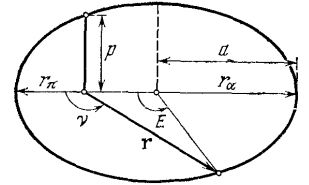
\includegraphics[width=0.35\textwidth]{Orbit_2D}
  \caption{Кеплерова эллиптическая орбита}
  \label{fig:KeplerOrbit2D}
\end{wrapfigure}
Величины $p$ и $e$ можно выразить через апогейное
($r_{\alpha}$) и перигейное ($r_{\pi}$) расстояния:
\begin{equation}
  p = \frac{2r_{\alpha}r_{\pi}}{r_{\alpha} + r_{\pi}},
  e = \frac{r_{\alpha} - r_{\pi}}{r_{\alpha} + r_{\pi}}.
\end{equation}
Наибольший размер эллипса характеризуется его большой полуосью $a$, при этом
\begin{equation}
  a = \frac{1}{2}(r_{\alpha} + r_{\pi}),
\end{equation}
а между $p$, $e$, $a$ существует связь
\begin{equation}
  p = a(1 - e^2).
\end{equation}
Угол $\nu$ в формуле \label{eq:GRENu} называется истинной аномалией.\par
Зависимость $\nu(t)$ от времени дает закон движения спутника по орбите. В теории
кеплеровских орбит наиболее трудное место -- отыскание явного выражения через время
$t$. Угловая скорость $d\nu/dt$ движения по орбите удовлетворяет так называемому
интегралу (или закону) площадей
\begin{equation} \label{eq:GIntegralSquares}
  r^2\frac{d\nu}{dt} = \sqrt{\mu p}.
\end{equation}\par
Если сюда подставить выражение $r(\nu)$ из (\ref{eq:GRENu}) и вычислить соответствующую
квадратуру, то получим явное выражение времени через $\nu: t = t(\nu)$. Задача состоит
в решении этого трансцендентного уравнения относительно $\nu$. Для этого вводится
новая переменная $E$, называемая эксцентрической аномалией (смысл ее виден на
рисунке \ref{fig:KeplerOrbit2D}) и связанная с $\nu$ соотношениями
\begin{equation}
  \cos\nu = \frac{\cos E - e}{1 - e\cos E}, \sin\nu = \frac{\sin E}{1 - e\cos E}\sqrt{1 - e^2},
\end{equation}
причем
\begin{equation}\label{eq:rFromEA}
  r = a(1 - e\sin E).
\end{equation}
Эксцентрическая аномалия $E$ связана со временем уравнением Кеплера:
\begin{equation} \label{eq:EscentricAnomaly}
  E - e\sin E = n(t-\tau^*),
\end{equation}
где $n = \sqrt{\mu/a^3}$ -- так называемое среднее движение; постоянная $\tau^*$
обозначает момент прохождения через перигей орбиты. Из (\ref{eq:EscentricAnomaly})
следует, что период обращения спутника по орбите
\begin{equation}
  T = 2\pi\sqrt{a^3/\mu}.
\end{equation}\par
Уравнение (\ref{eq:EscentricAnomaly}) не решается аналитически, поэтому для её
вычисления будем использовать один из алгоритмов численного решения уравнений, к примеру,
метод Эйлера:
\begin{equation}
  \begin{aligned}
    & E_{k+1} = e\sin E_k + M, \\
    & M = n(t - \tau^*).
  \end{aligned}
\end{equation}\par
Тем самым, положение спутника в каждый момент времени в плоскости орбиты
будет вычисляться по формуле:
\begin{equation}
  \begin{aligned}
    & \vec{r}_{orbital} = r \cdot [\cos\nu, \sin\nu, 0]^{T}, \\
    & r = a(1 - e\sin E)
  \end{aligned}
\end{equation}\par
Совершим переход из движения в плоскости орбиты к движению в пространстве, определив
компоненты фиксирующие положение орбиты в нем.
\begin{wrapfigure}{r}{0.35\textwidth}
  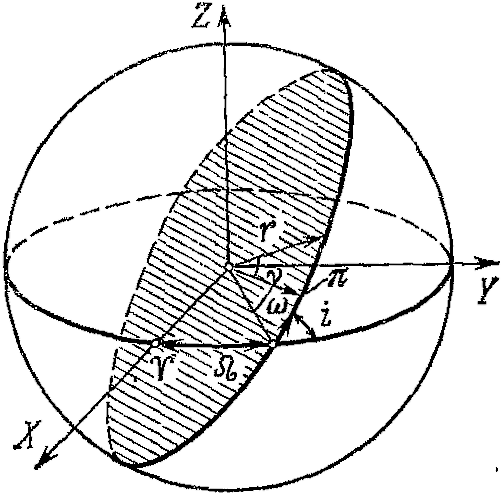
\includegraphics[width=\linewidth]{Orbit_Kepler.png}
  \caption{Кеплеровы элементы}
  \label{fig:KeplerOrbitParameters}
\end{wrapfigure}
Это положение описывают следующим образом (рисунок \ref{fig:KeplerOrbitParameters}).
Спроектируем плоскость орбиты на небесную сферу и рассмотрим систему координат $XYZ$
такую, что ось $Z$ направлена на Северный полюс мира (вполне определенная точка
на небесной сфере вблизи Полярной звезды), ось $X$ -- на точку весеннего
равноденствия (тоже вполне определенная точка); начало координат совпадает с
центром Земли, а плоскость $XY$ -- с плоскостью земного экватора.
Вводятся такие переменные, как долгота восходящего узла ($\Omega$), наклонение ($i$),
аргумент перигея ($\omega$).\par
Обобщив это, получим, что орбита спутника характеризуется двумя независимыми постоянными
параметрами: $p$ и $e$; положение орбиты в пространстве определяется тремя независимыми
углами: $\Omega$, $\omega$, $i$; положение спутника на орбите в каждый момент времени
определяется параметром $\tau^*$. Итак, имеем шесть независимых параметров, полностью
определяющих движение спутника в пространстве (его координаты и скорость в каждый
момент времени), например:
\begin{equation} \label{eq:KeplerOrbitalElements}
  p,\,\, e,\,\, \Omega,\,\, \omega,\,\, i,\,\, \tau^*
\end{equation}
Параметры (\ref{eq:KeplerOrbitalElements}) называются кеплеровыми элементами
орбиты спутника.
И положение спутника в пространстве в каждый момент времени будет вычисляться по формуле:
\begin{equation}
  \begin{aligned}
    & \vec{r} = R_z(\omega)R_x(i)R_z(\Omega) \cdot \vec{r}_{orbital}, \\
    & \vec{r}_{orbital} = r \cdot [\cos\nu, \sin\nu, 0]^{T}, \\
    & r = a(1 - e\sin E),
  \end{aligned}
\end{equation}\par
где $R_x$, $R_z$ -- матрицы поворота, выраженные следующим образом:
\begin{equation}
    \begin{aligned}
        &R_x(\phi) = \begin{bmatrix}
           1        &  0        &   0        \\
           0        &  \cos\phi &  -\sin\phi \\
           0        &  \sin\phi &   \cos\phi
        \end{bmatrix},\,\,
        R_y(\phi) = \begin{bmatrix}
           \cos\phi &  0        &  \sin\phi \\
           0        &  1        &  0        \\
          -\sin\phi &  0        &  \cos\phi
        \end{bmatrix},\,\, \\
        &R_z(\phi) = \begin{bmatrix}
          \cos\phi & -\sin\phi & 0 \\
          \sin\phi &  \cos\phi & 0 \\
          0        &  0        & 1
        \end{bmatrix}.
    \end{aligned}
\end{equation}
%
\section{Возмущенное движение. Оскулирующие элементы}
\noindent\indent Кеплерово движение, рассмотренное в предыдущем пункте, называют
ещё невозмущенным движением спутника. На самом же деле, при движении спутника под
действием возмущающих сил, кеплеровы элементы орбиты перестают быть постоянными,
и меняются со временем:
\begin{equation} \label{eq:KeplerOrbitalElementsTime}
  p(t),\,\, e(t),\,\, \Omega(t),\,\, \omega(t),\,\, i(t),\,\, \tau^*(t).
\end{equation}\par
Задача сводится тогда к отысканию явных зависимостей (\ref{eq:KeplerOrbitalElementsTime})
от времени.\par
<<Эллипс>> с переменными элементами (\ref{eq:KeplerOrbitalElementsTime}) называется
оскулирующим эллипсом, а сами переменные элементы -- оскулирующими элементами.\par
Чтобы составить дифференциальные уравнения для оскулирующих элементов (\ref{eq:KeplerOrbitalElementsTime}),
надо перейти от переменных $x$, $y$, $z$, $\dot{x}$, $\dot{y}$, $\dot{z}$ к переменным
(\ref{eq:KeplerOrbitalElementsTime}), подставить в уравнения (\ref{eq:GAccelerationModify})
и разрешить их относительно производных $\frac{dp}{dt}$, $\frac{de}{dt}$, $\frac{d\Omega}{dt}$,
$\frac{d\omega}{dt}$, $\frac{di}{dt}$, $\frac{d\tau^*}{dt}$ оскулирующих элементов.
\section{Уравнения в оскулирующих элементах}
\noindent\indent Ссылаясь на уже упомянутый труд В. В. Белецкого, приведем систему уравнений
в оскулирующих элементах орбиты:
\begin{equation}\label{eq:OsculirDynamic}
  \begin{cases}
    \frac{dp}{dt} = 2r\sqrt{\frac{p}{\mu}}T, \\
    \frac{de}{dt} = \sqrt{\frac{p}{\mu}}\left\{
      S\sin\nu + T\left[(1 + \frac{r}{p})\cos\nu + e\frac{r}{p}\right]
    \right\}, \\
    \frac{d\omega}{dt} = \frac{1}{e}\sqrt{\frac{p}{\mu}}\left[
      -S\cos\nu + T(1 + \frac{r}{p})\sin\nu - W e\frac{r}{p}\sin u\ctg i
    \right] \\
    \frac{di}{dt} = W \frac{r}{\sqrt{\mu p}}\cos u, \\
    \frac{d\Omega}{dt} = W \frac{r}{\sqrt{\mu p}}\frac{\sin u}{\sin i}, \\
    \frac{d\tau^*}{dt} = \frac{r^2}{e\mu}\left[
      S (eN\sin\nu - \cos\nu) + T N\frac{p}{r}
    \right],
  \end{cases}
\end{equation}\par
\noindent здесь
\begin{equation}
    \begin{aligned}
    &N = \frac{p^2}{r^2}\int\limits_0^{\nu} \frac{2\cos\nu}{(1 + e\cos\nu)^3}d\nu;\\
    &u = \nu + \omega;
    \end{aligned}
\end{equation}\par
$S$, $T$, $W$ -- соответственно радиальное, трансверсальное и нормальное возмущающие
ускорения.\par
\begin{figure}[h]
  \centering
  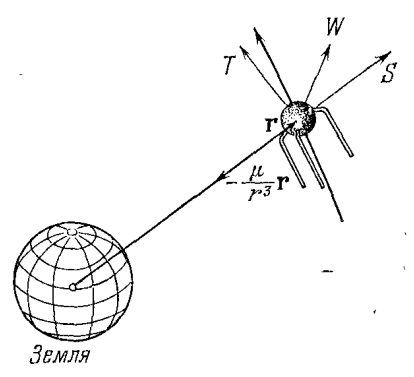
\includegraphics[width=0.35\textwidth]{ForcesOrientation}
  \caption{Система координат}
  \label{fig:ForcesOrientation}
\end{figure}\par
\section{Возмущения от зональных гармоник}
\noindent\indent Сила ньютоновского притяжения и соответствующая силовая функция
лишь приближенно описывают силу притяжения, действующую на спутник со стороны
реальной Земли. Однако, в виду <<сплюснутости>> в направлении полюсов (и в малой
степени также и <<с боков>>), не совсем симметрична, неоднородна, в результате
чего поле сил, создаваемое Землей, имеет довольно сложную структуру. Для более
хорошего приближения к реальному полю сил представляют силовую функцию в следующем виде:
\begin{equation} \label{eq:UModifiy}
  U = \frac{\mu}{r}\left\{1 + \sum\limits_{k=2}^{\infty}I_k\left(\frac{R}{r}\right)^kP_k(\sin\phi)\right\},\,\,
  \mu = GM,
\end{equation}
где $M$ -- масса Земли;

$G$ -- универсальная постоянная тяготения;

$R$ -- экваториальный радиус Земли;

$\phi$ -- географическая широта точки (отстоящей от центра Земли на
расстоянии $r$).

Коэффициенты $I_k$ имеют фиксированные безразмерные значения.
Функции $P_k$ представляют собой полиномы Лежандра, определяемые следующим образом:
\begin{equation}
  \begin{cases}
    \begin{aligned}
      & P_0(x) = 1, \\
      & P_1(x) = x, \\
      & P_2(x) = \frac{1}{2}(3x^2 - 1), \\
      & P_3(x) = \frac{1}{2}(5x^3 - 3x), \\
      & ...\\
      & P_n(x) = \frac{1}{2^n \cdot n!}\frac{d^n}{dx^n}(x^2 - 1)^n, \\
    \end{aligned}
  \end{cases}
\end{equation}\par
Таким образом, силовая функция (\ref{eq:UModifiy}) зависит только от расстояния
до центра притяжения, как силовая функция, но ещё и от широты места. Силовая
функция предполагает, что поле сил осесимметрично (относительно оси, проходящей
через полюсы Земли). Видим, что (\ref{eq:UModifiy}) представляет собой сумму
ньютоновского потенциала и добавочных членов, которые, по определению возмущений,
должны быть малы по сравнению с основным (первым) членом. Действительно,
коэффициенты $I_k$ в (\ref{eq:UModifiy}) имеют такие значения:
\begin{equation}
  \begin{cases}
    \begin{aligned}
      & I_2 = -1082.2\cdot10^{-6}, \\
      & I_3 = 2.3\cdot10^{-6}, \\
      & I_4 = 2.1\cdot10^{-6}, \\
      & ...,
    \end{aligned}
  \end{cases}
\end{equation}
так что даже самый большой из этих коэффициентов $I_2$ дает добавку порядка
десятой доли процента, а остальные коэффициенты -- ещё на несколько порядков
меньше. Коэффициент $I_2$ характеризует наиболее существенное отличие поля
тяготения реальной Земли от идеальной шаровой.\par
Рассмотрим влияние основного возмущения на движение спутника в поле тяготения Земли.
Итак, возмущающая силовая функция
\begin{equation}
  U = \frac{\mu}{r}I_2\left(\frac{R}{r}\right)^2 \frac{1}{2}(3\sin^2\phi - 1).
\end{equation}\par
  Для записи возмущающего ускорения, вызванного не центральностью гравитационного
поля Земли, на оси орбитальной системы координат воспользуемся соотношениями,
вытекающими из рисунка \ref{fig:GarmonicOrbitalEq}.\par
  На этом рисунке положение спутника характеризуется точкой A; плоскость орбиты
спутника есть EAF; меридиональная плоскость, проходящая через точку A, - BCD.
Угол между местным меридианом и трансверсальным направлением в точку A обозначен
$\psi$, угол ECA - $u$ (аргумент широты), угол ABC -- $\phi$ -- широта точки.
\begin{figure}[h]
  \centering
  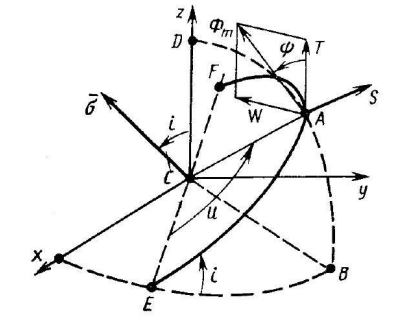
\includegraphics[width=0.35\textwidth]{GarmonicOrbitalEq}
  \caption{Проекции возмущающих ускорений в орбитальной системе координат}
  \label{fig:GarmonicOrbitalEq}
\end{figure}\par
Легко получить соотношения (\ref{eq:GarmonicOrbitalAcceleration}):\par
\begin{equation} \label{eq:GarmonicOrbitalAcceleration}
  \begin{aligned}
    & S = \frac{3I_2\mu R^2}{2r^4} \cdot (3\sin^2\phi - 1) = \frac{3I_2\mu R^2}{2r^4} \cdot (3\sin^2 i\sin^2 u - 1), \\
    & T = \frac{3I_2\mu R^2}{2r^4} \cdot (\sin2\phi\cos\psi) = - \frac{3I_2\mu R^2}{2r^4} \cdot (\sin^2 i\sin2 u), \\
    & W = \frac{3I_2\mu R^2}{2r^4} \cdot (\sin2\phi\sin\psi) = -\frac{3I_2\mu R^2}{2r^4} \cdot (\sin2 i\sin u), \\
  \end{aligned}
\end{equation}\par
При выводе последних равенств были использованы следующие формулы сферической
тригонометрии:
\begin{equation}
  \sin\phi = \sin u \sin i,\,\, \cos\psi = \ctg u \tg\phi,
\end{equation}
где $i$ -- наклонение орбиты, $u$ -- аргумент широты.
\section{Аэродинамическое сопротивление}
\noindent\indent Одни из наиболее влияющих на движение низкоорбитальных спутников
(т.е. спутников, движущихся на высотах от 150 до 1500 км) сил негравитационной
природы оказываются аэродинамические силы, вызванные влиянием атмосферы Земли.\par
    Сила, действующая на парус, при сопротивлении атмосферы, записывается в
следующем виде:
\begin{equation}
    \vec{F}_{\text{a}} = -\frac{C_d A}{2}\rho|\vec{v}_{\text{отн}} \cdot \vec{n}| \vec{v}_{\text{отн}},
\end{equation}
где $C_d$ -- коэффициент лобового сопротивления (принимаем равным стандартному
значению $2.2$), $\rho$ -- плотность атмосферы, $\vec{v}_{\text{отн}}$ --
скорость КА с парусом относительно набегающего потока. Для простоты рассчитываем
последнее в приближении плотностью увлекаемой Землей атмосферы
\begin{equation}
    \vec{v}_{\text{отн}} = \vec{v} - \vec{\omega}_{\oplus} \times \vec{r} =
\sqrt\frac{\mu}{p}\begin{bmatrix}
           e_x\sin u - e_y\cos u \\
           1 + e_x\cos u + e_y\sin u \\
           0
         \end{bmatrix} - \omega_{\oplus}r\begin{bmatrix}
                    0 \\
                    \cos i \\
                    \sin i \cos u
                  \end{bmatrix},
\end{equation}
где $\omega_{\oplus} \approx 7.29\cdot 10^{-5} \text{с}^{-1}$ -- скорость вращения
Земли вокруг своей оси.\par
    Также запишем выражения для аэродинамического момента:
\begin{equation}
    \vec{M}_{\text{a}} = \frac{C_d A}{2}\rho|\vec{v}_{\text{отн}} \cdot \vec{n}| \vec{v}_{\text{отн}}\times\vec{r}
\end{equation}
\section{Давление солнечного света}
\noindent\indent Сила светового давления включает в себя несколько составляющих:
давление от поглощенного излучения, отраженного, пропущенного, а также собственное
излучение паруса. Данные факторы зависят от соответствующих оптических характеристик --
коэффициентов поглощения, отражения, пропускания и излучательной способности. В
общем случае данные факторы зависят от направления в пространстве, свойств поверхности,
длины волны, температуры поверхности и др.\par
  Предполагая начальную (раскройную) форму поверхности солнечного паруса плоской,
введем прямоугольную декартову систему координат $Ox_1x_2x_3$ на раскройной форме
солнечного паруса (рисунок \ref{fig:SailCoordinateSystem}). Деформированное состояние
паруса зададим через поле векторов перемещения точек полотна паруса
$\vec{u} = (u_1, u_2, u_3)^T$. Зададим единичный вектор нормали $\vec{n}$,
положительное направление которого определено для освещенной стороны полотна паруса.
\begin{figure}[h]
  \centering
  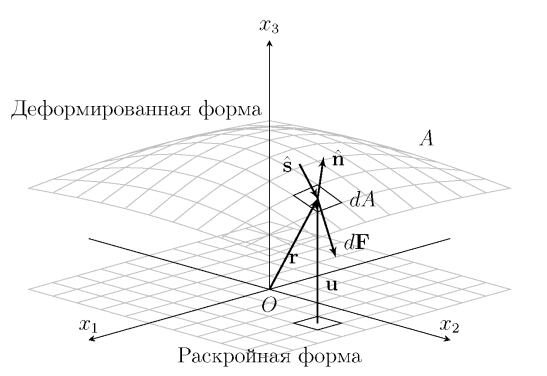
\includegraphics[width=0.5\textwidth]{SailCoordinateSystem}
  \caption{Раскройная форма солнечного паруса}
  \label{fig:SailCoordinateSystem}
\end{figure}
Определим единичный вектор $\vec{s}$, направленный от источника света на полотно
паруса. На достаточно большом удалении от Солнца вектор $\vec{s}$ можно считать
постоянным для всей поверхности солнечного паруса.\par
  Запишем элементарную силу светового давления как
\begin{equation}
  d\vec{F}_{\text{SRP}} = P(R) \cdot \left[
    -a_{1}(\vec{n}\cdot\vec{s})\vec{s}
    +a_{2}(\vec{n}\cdot\vec{s})\vec{n}
    -2a_{3}(\vec{n}\cdot\vec{s})^2\vec{n}
  \right]dA,
\end{equation}
здесь
\begin{equation}
  P(R) = \frac{q_0(R)}{c}
\end{equation}
-- световое давление ($q_0(R)$ -- солнечная постоянная, которая зависит от
расстояния $R$ до Солнца, $c$ -- скорость света в вакууме), что на относительно
близких дистанциях от Земли равна $4.56\cdot 10^{-6} \text{H}/\text{м}^2$;

$a_{1}$, $a_{2}$, $a_{3}$ -- обобщенные оптические параметры, определяемые
следующим образом:
\begin{equation}
  \begin{aligned}
    & a_{1} = 1 - \rho s, \\
    & a_{2} = B_f\rho(1 - s) + (1 - \rho)\frac{\epsilon_f B_f - \epsilon_b B_b}{\epsilon_f + \epsilon_b}, \\
    & a_{3} = \rho s, \\
  \end{aligned}
\end{equation}
причем $\rho$ -- коэффициент зеркального отражения; $s$ -- коэффициент зеркальности;
$B_f$ и $B_b$ -- коэффициенты, показывающие характер индикатрисы отражения за вычетом
зеркальной составляющей (в случае диффузного отражения $B = 2/3$); $e_f$ и $e_b$ --
излучательная способность освещенной и обратной стороны паруса.\par
  Параметры $a_{1}$ и $a_{3}$ учитывают зеркальную составляющую, а первое слагаемое
параметра $a_{2}$ в случае, когда $B_f$ и $B_b = 2/3$, -- диффузную составляющую.
Второе слагаемое параметра $a_{2}$ отвечает за вклад собственного теплового излучения
полотна в результирующую силу светового давления.\par
  Аналогично запишем выражения для момента от элементарной силы светового давления
\begin{equation}
  d\vec{M}_{\text{SRP}} = P(R) \cdot \left[
    -a_{1}(\vec{n}\cdot\vec{s})(\vec{r} \times \vec{s})
    +a_{2}(\vec{n}\cdot\vec{s})(\vec{r} \times \vec{n})
    -2a_{3}(\vec{n}\cdot\vec{s})^2(\vec{r} \times \vec{n})
  \right]dA,
\end{equation}
где $\vec{r}$ -- вектор, задающий положение элементарной площадки $dA$.\par
  Векторы $\vec{s}$ и $\vec{n}$ задаются в ОСК выражениями\par
\begin{equation} \label{eq:SunVector}
  \vec{s} = \begin{bmatrix}
     \sin\psi_s\sin\theta_s \\
    -\cos\psi_s\sin\theta_s \\
     \cos\theta_s
  \end{bmatrix},
\end{equation}
\begin{equation}
  \vec{n} = \begin{bmatrix}
     \sin\psi\sin\theta \\
    -\cos\psi\sin\theta \\
     \cos\theta
  \end{bmatrix}.
\end{equation}\par
Связь компонент вектора Солнца $\vec{s}$ с положением плоскости орбиты относительно
направления на Солнце выявляется из сравнения (\ref{eq:SunVector}) и альтернативного
выражения
\begin{equation}
  \vec{s} = \begin{bmatrix}
    \sigma_x\cos u + \sigma_y\sin u \\
    \sigma_y\cos u - \sigma_x\sin u \\
    \sigma_z
  \end{bmatrix}
\end{equation}
через компоненты вектора $\sigma$, связанные с долготой восходящего узла $\Omega$,
наклонением $i$ и эклиптической долготой $\lambda$ по формуле
\begin{equation}
\begin{aligned}
    & \sigma_x =  \cos\Omega\cos\lambda + \sin\Omega\sin\lambda\cos\epsilon, \\
    & \sigma_y =  \cos\Omega\cos i\sin\lambda\cos\epsilon - \sin\Omega\cos i\cos\lambda + \sin i\sin\lambda\sin\epsilon, \\
    & \sigma_z = -\cos\Omega\sin i\sin\lambda\cos\epsilon + \sin\Omega\sin i\cos\lambda + \cos i\sin\lambda\sin\epsilon,
\end{aligned}
\end{equation}
где $\epsilon = 23^o26'$ -- наклон эклиптики к экватору. Имеем:
\begin{equation}
  \begin{aligned}
    & \theta_s = \arccos\sigma_z, \\
    & \psi_s = atan2(\sigma_x\cos u + \sigma_y\sin u, \sigma_x\sin u - \sigma_y\cos u).
  \end{aligned}
\end{equation}
Функция $atan2$ обозначает операцию взятия обратного тангенса с учетом знаков
обоих аргументов.
\section{Теневая зона орбиты}
\noindent\indent Для учета нахождения космического аппарата в области тени и
полутени вводят, так называемую, <<функцию тени>>, что представляет собой
скалярную функцию, зависящую от положения спутника относительно Земли и Солнца.
\begin{wrapfigure}{r}{0.35\textwidth}
  \centering
  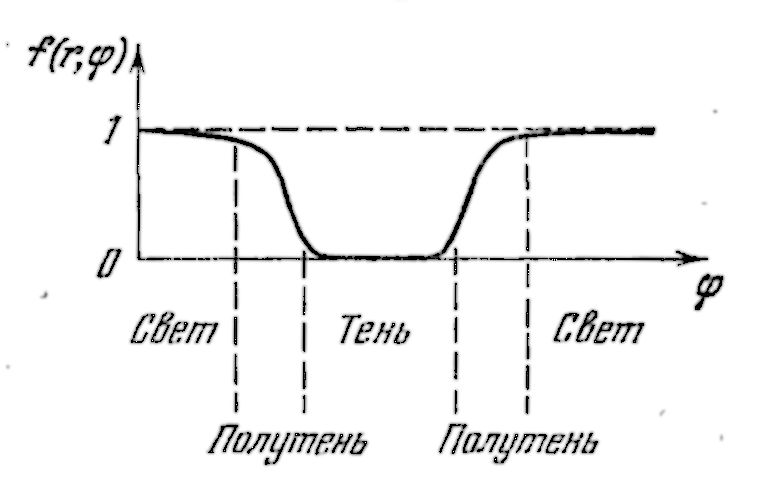
\includegraphics[width=0.35\textwidth]{shadowFunction}
  \caption{Функция тени}
  \label{fig:shadowFunction}
\end{wrapfigure}
Ввиду сложности эффекта отбрасывания тени Землей и нечеткости границы полутени,
в качестве функции тени часто берется не <<релейная>>, непрерывная, функция,
аппроксимирующую реальные свойства тени, типа функции, изображенной на
рисунке \ref{fig:shadowFunction}.
Где $r$ -- вектор, направленный от центра Земли к центру масс спутника; $\phi$
-- угол между вектором, направленным вдоль вектора, пущенного из центра Солнца к
центру Земли и вектором $r$.\par
Рассмотрим график нахождения спутника в плоскости $xOy$ (рисунок \ref{fig:EarthShadow}),
где в качестве центра системы координат возьмем центр Солнца; ось $OX$ направлена
вдоль вектора, направленного из центра Солнца к центру Земли ($\vec{r}_{SE}$);
ось $OY$ лежит в плоскости, образованной векторами $\vec{r}_{SE}$ и $\vec{r}$ и направлена
вдоль вектора $(\vec{r}\times\vec{r}_{SE})\times\vec{r}$.
\begin{figure}[!h]%{r}{0pt}
  \centering
  \begin{tikzpicture}[thick,scale=0.6, every node/.style={transform shape}]
    \coordinate (Sun) at (0,0);
    \coordinate (Earth) at (16,0);
    \coordinate (Y) at (0,4);
    \coordinate (X) at (24,0);
    \coordinate (YDot) at (16,4);

    \draw[thick, ->] (-4, 0) -- (X) node[below] {$x$};
    \draw[thick, ->] (0, -4) -- (Y) node[left] {$y$};

    \draw[yellow, thick] (Sun) circle (3);
    \draw[->] (Sun) -- node[left] {$R_{Sun}$} (-2.1213203435596424, -2.1213203435596424);

    \draw[thick, ->] (Sun) -- node[below] {$\vec{r}_{SE}$} (Earth);

    \draw[thick, ->] (Earth) -- (16, 4) node[left] {$y'$};
    \draw[thick] (Earth) -- (16, -4);

    \draw[blue, thick] (Earth) circle (1);
    \draw[->] (Earth) -- node[right] {$R_{Earth}$} (15.292893218813452, -0.7071067811865475);

    \draw[thick, dashed, red] (Earth) circle (2);

    % спутник
    \draw[thick, ->] (Earth) -- (16.5176380902050415, 1.9318516525781366)  node[right] {$\vec{r}$};
    % угол спутника
    \draw (17.3, 0) arc (0:75:1.3) node[right] {$\phi$};

    % полутень
    \draw[thick, dashed] (0, 3) -- (24, -3);
    \draw[thick, dashed] (0, -3) -- (24, 3);
    \draw (0.7, -2.8) arc (20:90:0.7) node[right] {$\omega_{\text{пт}}$};
    % угол полутени
    \coordinate (Shadow2) at (17.461435894335995, 1.3653589735839988);
    \draw (16.7, 0) arc (0:45:0.7) node[right] {$\phi_{\text{пт}}$};
    \draw (16, 0) -- (Shadow2);

    % тень
    \draw[thick, dashed] (0, 3) -- (24, 0);
    \draw[thick, dashed] (0, -3) -- (24, 0);
    \draw (0.7, 2.9) arc (-15:-90:0.7) node[right] {$\omega_{\text{т}}$};
    % угол тени
    \draw (16.3, 0) arc (0:22.5:0.3) node[right] {$\phi_{\text{т}}$};
    \coordinate (Shadow) at (17.846153846153847, 0.7692307692307692);
    \draw (16, 0) -- (Shadow);
  \end{tikzpicture}
  \caption{Образование теневых зон}
  \label{fig:EarthShadow}
\end{figure}\par
Здесь $R_{Sun}$ -- радиус Солнца; $R_{Earth}$ -- радиус Земли;
$\omega_{\text{т}}$; $\omega_{\text{пт}}$  -- вспомогательные углы, образующие
коническую поверхность областей тени и полутени; $\phi$ -- угол между вектором
$\vec{r}$ и $\vec{r}_{SE}$; $\phi_{\text{т}}$, $\phi_{\text{пт}}$ -- углы,
характеризующие линии раздела областей тени и полутени.\par
Угол $\phi$ находится через скалярное произведение векторов $\vec{r}$ и $\vec{r}_{SE}$
\begin{equation}
\vec{r} \cdot \vec{r}_{SE} = |\vec{r}||\vec{r}_{SE}|\cos\phi,
\end{equation}
тем самым, получим угол $\phi$
\begin{equation}
\phi = \arccos\frac{\vec{r} \cdot \vec{r}_{SE}}{|\vec{r}||\vec{r}_{SE}|}.
\end{equation}\par
Углы $\omega_{\text{т}}$; $\omega_{\text{пт}}$ выводятся из следующих выражений:
\begin{equation}
\tg\omega_{\text{т}} = \frac{R_{Sun} - R_{Earth}}{r_{SE}},\,\,
\tg\omega_{\text{пт}} = \frac{R_{Sun} + R_{Earth}}{r_{SE}}.
\end{equation}
\par
Найдем углы $\phi_{\text{т}}$, $\phi_{\text{пт}}$, решив системы уравнений,
описывающих линии раздела областей тени, полутени и области без тени.\par
\begin{equation}
(1): \begin{cases}
y = R_{Sun} - \tg\omega_{\text{т}} \cdot x, \\
y^2 + (x - r_{SE})^2 = r^2, \\
y = \tg\phi_{\text{т}} \cdot (x - r_{SE}),
\end{cases}
(2): \begin{cases}
y = - R_{Sun} + \tg\omega_{\text{пт}} \cdot x, \\
y^2 + (x - r_{SE})^2 = r^2, \\
y = \tg\phi_{\text{пт}} \cdot (x - r_{SE}),
\end{cases}
\end{equation}\par
Решим первую систему, первоначально найдя крайнюю правую точку пересечения линии раздела областей
и орбиты спутника.\par
\begin{equation}
\begin{aligned}
 &\begin{cases}
  y = R_{Sun} - \tg\omega_{\text{т}} \cdot x, \\
  (R_{Sun} - \tg\omega_{\text{т}} \cdot x)^2 + (x - r_{SE})^2 = r^2, \\
  y = \tg\phi_{\text{т}} \cdot (x - r_{SE}),
\end{cases} \\
&\begin{cases}
  y = R_{Sun} - \tg\omega_{\text{т}} \cdot x, \\
  R_{Sun}^2 - 2 R_{Sun} \tg\omega_{\text{т}} \cdot x + \tg^2\omega_{\text{т}} \cdot x^2
  + x^2 - 2 r_{SE} x + r^2_{SE} = r^2, \\
  y = \tg\phi_{\text{т}} \cdot (x - r_{SE}),
\end{cases} \\
&\begin{cases}
  y = R_{Sun} - \tg\omega_{\text{т}} \cdot x, \\
  (\tg^2\omega_{\text{т}} + 1) \cdot x^2
  - 2 (r_{SE} + R_{Sun} \tg\omega_{\text{т}}) \cdot x
  + (R_{Sun}^2 + r^2_{SE} - r^2) = 0, \\
  y = \tg\phi_{\text{т}} \cdot (x - r_{SE}),
\end{cases} \\
& D/4 = (r_{SE} + R_{Sun} \tg\omega_{\text{т}})^2 -
(\tg^2\omega_{\text{т}} + 1) (R_{Sun}^2 + r^2_{SE} - r^2), \\
& D/4 = (\tg^2\omega_{\text{т}} + 1)r^2 - (R_{Sun}^2 - 2R_{Sun}r_{SE}\tg\omega_{\text{т}} + r^2_{SE}\tg^2\omega_{\text{т}}), \\
& D/4 = (\tg^2\omega_{\text{т}} + 1)r^2 - (R_{Sun} - r_{SE}\tg\omega_{\text{т}})^2, \\
& x = \frac{
  r_{SE} + R_{Sun} \tg\omega_{\text{т}} \pm \sqrt{(\tg^2\omega_{\text{т}} + 1)r^2 - (R_{Sun} - r_{SE}\tg\omega_{\text{т}})^2}
}{\tg^2\omega_{\text{т}} + 1}, \\
& \begin{cases}
  y_{\text{т}} = R_{Sun} - \tg\omega_{\text{т}} \cdot x_{\text{т}}, \\
  x_{\text{т}} = \frac{
    r_{SE} + R_{Sun} \tg\omega_{\text{т}} + \sqrt{(\tg^2\omega_{\text{т}} + 1)r^2 - (R_{Sun} - r_{SE}\tg\omega_{\text{т}})^2}
  }{\tg^2\omega_{\text{т}} + 1},
\end{cases}
\end{aligned}
\end{equation}\par
Получив точку пересечения, выведем угол $\phi_{\text{т}}$:
\begin{equation}
\begin{aligned}
& \begin{cases}
  \phi_{\text{т}} = \arctg\frac{y_{\text{т}}}{x_{\text{т}} - r_{SE}}, \\
  y_{\text{т}} = R_{Sun} - \tg\omega_{\text{т}} \cdot x_{\text{т}}, \\
  x_{\text{т}} = \frac{
    r_{SE} + R_{Sun} \tg\omega_{\text{т}} + \sqrt{(\tg^2\omega_{\text{т}} + 1)r^2 - (R_{Sun} - r_{SE}\tg\omega_{\text{т}})^2}
  }{\tg^2\omega_{\text{т}} + 1},
\end{cases}
\end{aligned}
\end{equation}\par
Аналогично выводится угол полутени $\phi_{\text{пт}}$. Так как при подстановке уравнения
линии раздела в уравнение окружности теряется знак и получается аналогичное уравнение,
отличающееся от вышеописанного тем, что используется тангенс угла наклона $\omega_{\text{пт}}$,
вместо $\omega_{\text{т}}$.\par
Опустив выкладку, напишем формулу вычисления угла полутени:
\begin{equation}
\begin{aligned}
& \begin{cases}
  \phi_{\text{пт}} = \arctg\frac{y_{\text{пт}}}{x_{\text{пт}} - r_{SE}}, \\
  y_{\text{пт}} = - R_{Sun} + \tg\omega_{\text{пт}} \cdot x_{\text{пт}}, \\
  x_{\text{пт}} = \frac{
    r_{SE} + R_{Sun} \tg\omega_{\text{пт}} + \sqrt{(\tg^2\omega_{\text{пт}} + 1)r^2 - (R_{Sun} - r_{SE}\tg\omega_{\text{пт}})^2}
  }{\tg^2\omega_{\text{пт}} + 1},
\end{cases}
\end{aligned}
\end{equation}\par
В первом приближении, можно использовать в качестве функции тени, следующую модель:
\begin{equation}
f(r, \phi) = \begin{cases}
0, & \phi < \phi_{\text{т}}, \\
0.5, & \phi_{\text{т}} < \phi < \phi_{\text{пт}}, \\
1, & \phi > \phi_{\text{пт}},
\end{cases}
\end{equation}
однако, в таком случае переход из одного состояние в другое не будет плавным, поэтому
вводятся различные модели плавного перехода из одной области в другую. В данной работе,
используется <<сигмоид>> следующего вида:
\begin{equation}
  f(\phi, \phi_{\text{пт}}, \phi_{\text{т}}) = \frac{1}{1 + e^{-2\frac{\phi - \phi_{\text{т}}}{\phi_{\text{пт}} - \phi_{\text{т}}}}}.
\end{equation}
Тогда ускорение, приобретаемое телом под действием силы солнечного давления, примет
следующий вид:
\begin{equation}
  \vec{f}_{\text{SRP}} = \frac{\vec{F}_{\text{SRP}}}{m} \cdot f(\phi, \phi_{\text{пт}}, \phi_{\text{т}}).
\end{equation}
\chapter{Рассмотрение задачи поиска оптимальных параметров ориентации}
\section{Оптимальное управление}
\noindent\indent В рассматриваемой задаче увода спутника на более высокую орбиту,
целевая функция выглядит следующим образом:
\begin{equation} \label{eq:IntMaxFullEq}
  \argmax\limits_{\alpha(t),\,\beta(t),\,\gamma(t)}\int\limits_{t_0}^{t_1} r dt,
\end{equation}\par
    где $r$ -- расстояние от центра Земли до центра масс спутника;\par
    $\alpha(t),\,\beta(t),\,\gamma(t)$ -- оптимальные функции углов ориентации
спутника относительно орбитальной системы координат.\par
    Как уже описывалось выше, положения спутника в пространстве характеризуется
кеплеровыми элементами орбиты, но характер самой орбиты описываются двумя параметрами:
параметром орбиты ($p$) и эксцентриситетом ($e$). Не стоит забывать про параметры ориентации
орбиты, так как они отражают такую характеристику, как взаимное расположение спутника,
Земли и Солнца. Однако, данный эффект будет рассмотрен позднее.\par
    Расстояние от центра Земли до центра масс спутника рассчитывается из формулы
(\ref{eq:rFromEA}):
\begin{equation}
    r = a(1 - e\sin E).
\end{equation}\par
    Для упрощения вычисления целевой функции, возможно сменить подынтегральную
функцию длины радиус-вектора орбиты на значение большей полуоси орбиты,
убрав тем самым необходимость в пересчете эксцентрической аномалии.
\begin{equation} \label{eq:IntMaxFullEq}
  \argmax\limits_{\alpha(t),\,\beta(t),\,\gamma(t)}\int\limits_{t_0}^{t_1} a dt,
\end{equation}\par
где $a = \frac{p}{1 - e^2}$.\par
    В качестве ограничения на область допустимых значений углов ориентации, выступают
уравнения Эйлера (\ref{eq:EulerDynamic})-(\ref{eq:EulerKinematic}).
\section{Математические методы}
\noindent\indent Для поиска оптимальных управляющих углов в данной работе сравнивались
следующие подходы.
\subsection{Градиентный метод}
\noindent\indent Одним из простейших алгоритмов поиска решения для задачи локальной
оптимизации является метод градиентного спуска, суть которого заключается в следующем:\par
  Дана некоторая целевая функция вида:\par
\begin{equation}
  F(\vec{x}) : \mathbb{X} \rightarrow \mathbb{R},
\end{equation}
и задача оптимизации следующего вида:
\begin{equation}
  F(\vec{x}) \rightarrow \max\limits_{\vec{x}\in \mathbb{X}}.
\end{equation}
Предполагается, что функция $F \in C^1(\mathbb{X})$. Тогда, используя градиент
функции, можно итеративно приблизится к локальному максимуму функции из каждой точки,
вычисляя на каждом шаге новое приближение следующим образом:
\begin{equation}
  \vec{x}_{k+1} = \vec{x}_{k} + \lambda_{k} \nabla F,
\end{equation}
где $\lambda_{k}$ выбирается одним из следующих подходов:
\begin{itemize}
  \item постоянной величиной (метод может расходиться): $\lambda_{k} = \lambda$;
  \item дробным шагом: $\lambda_{k} = \lambda / g(k)$;
  \item наискорейшим спуском: $\lambda_{k} = \argmax\limits_{\lambda} F(\vec{x}_{k} + \lambda \nabla F)$.
\end{itemize}
\subsection{Генетический алгоритм}
\noindent\indent Более трудоемким является поиск решения через такой эвристический
подход, как использование генетического алгоритма.\par
  В общем виде алгоритм его работы представляет собой выполнение следующих операций:
\begin{enumerate}
  \item Создание начальной популяции,
  \item Отбор <<родителей>> для создания следующего поколения,
  \item Размножение (скрещивание),
  \item Мутация,
  \item Селекция нового поколения.
\end{enumerate}\par
  В условиях решаемой задачи, процесс поиска <<наиболее приспособленного>> гена,
реализован следующим образом:
  Первоначально задаются области допустимых значений:
\begin{equation}
    \phi \in G_{\phi},\,\, \theta \in G_{\theta},\,\, \gamma \in G_{\gamma},
\end{equation}
где $G_{\phi}$, $G_{\theta}$, $G_{\gamma}$ -- области допустимых значений углов.\par
    После создается начальная популяция, путем случайного подбора точек в области допустимых
значений:
\begin{equation}
  \begin{aligned}
    & \alpha_i,\, \beta_i,\, \gamma_i \leftarrow random(G_\phi),\, random(G_\theta),\, random(G_\gamma) \\
    & f_i \leftarrow F(\alpha_i,\, \beta_i,\, \gamma_i) \\
    & population.push(f_i \rightarrow \alpha_i,\, \beta_i,\, \gamma_i)
  \end{aligned}
\end{equation}
  Дальше происходит цикл формирования нового поколения.
\subsubsection{Первый этап. Отбор (селекция) родительского поколения.}
\noindent\indent На этапе отбора <<родителей>> нужно из всей популяции выбрать определённую её
долю, которая останется на этом этапе эволюции. Есть разные способы
проводить отбор. Вероятность выживания особи $h$ должна зависеть от значения функции
приспособленности $f(h)$. Сама доля от общей популяции $s$ обычно является параметром
генетического алгоритма, и её просто задают заранее. По итогам отбора из $N$ особей
популяции $population$ остаются $sN$ особей, которые в дальнейшем станут основой
для создания новой популяции. Есть несколько подходов применяемых для выбора
подходящих <<особей>>. Наиболее привлекательными являются следующие методы отбора:
\begin{itemize}
  \item Метод рулетки -- вероятность выбора особи тем выше, чем лучше значение
функции приспособленности и определяется по формуле $p_i = \frac{f_i}{\sum\limits_{k=1}^{N}f_k}$;
  \item Сигма отсечение -- вероятность выбора особи тем выше, чем оптимальнее
значение масштабируемой целевой функции $p_i = \frac{F_i}{\sum\limits_{k=1}^{N}F_k}$,
где $F_i = 1 + \frac{f_i - \overline{f}}{2\sigma}$, где $\overline{f}$ -- среднее
значение целевой функции для всей популяции, $\sigma$ -- с.к.о значения целевой функции.
\end{itemize}
\subsubsection{Второй этап. Размножение (скрещивание).}
\noindent\indent Размножение в генетических алгоритмах требует для производства потомка нескольких
родителей, обычно двух.\par
Можно выделить несколько операторов выбора родителей:
\begin{itemize}
  \item Панмиксия — оба родителя выбираются случайно, каждая особь популяции имеет
  равные шансы быть выбранной;
  \item Инбридинг — первый родитель выбирается случайно, а вторым выбирается тот,
  что наиболее похож на первого родителя;
  \item Аутбридинг — первый родитель выбирается случайно, а вторым выбирается тот,
  что наиболее не похож на первого родителя.
\end{itemize}\par
    Инбридинг и аутбридинг бывают в двух формах: фенотипной и генотипной. В случае
фенотипной формы похожесть измеряется в зависимости от значения функции приспособленности
(чем ближе значения целевой функции, тем особи более похожи), а в случае генотипной
формы похожесть измеряется в зависимости от представления генотипа (чем меньше
отличий между генотипами особей, тем особи похожее).
\subsubsection{Третий этап. Мутация}
\noindent\indent К мутациям относится все то же самое, что и к размножению: есть
некоторая доля мутантов среди особей вновь созданного поколения $m$, являющаяся
параметром генетического алгоритма, и на шаге мутаций нужно выбрать $mN$ особей,
а затем случайным образом изменить значения их <<хромосом>> в соответствии с заранее
определёнными операциями мутации.
\subsubsection{Четвертый этап. Селекция нового поколения}
\noindent\indent Из особей текущего поколения и вновь созданного поколения выбираются
наиболее <<приспособленные>> и становятся новым поколением для следующего цикла
алгоритма.
\subsection{Алгоритм Нелдера-Мида}
\noindent\indent Метод безусловной оптимизации функции от нескольких переменных,
не использующий производной функции.\par
  Суть метода заключается в последовательном перемещении и деформировании симплекса
вокруг точки экстремума, посредством следующих операций:\par
\begin{enumerate}
  \item Отражение (reflection);
  \item Растяжение (expansion);
  \item Внешнее сжатие (outside contraction);
  \item Внутреннее сжатие (inside contraction);
  \item Сокращение (shrink).
\end{enumerate}
Для каждой операции вводятся связанные с ними скалярные величины: $\alpha$ (reflection),
$\beta$ (expansion), $\gamma$ (contraction), $\delta$ (shrink).\par
  Метод использует концепцию симплекса, который представляется в виде специального
политопа с $n+1$ вершиной в $n$-мерном пространстве.\par
\subsubsection{Алгоритм}
\noindent\indent Необходимо минимизировать функцию $F(\vec{x})$ (для максимизации
берется функция $-F(\vec{x})$), где $\vec{x} \in \mathbb{R}^n$. На первом
шаге случайным образом выбирается $n+1$ случайная точка и формируется $n+1$-мерный
симплекс.\par
\paragraph{Частичный порядок}\par
\noindent\indent В каждой точке вычисляется значение функции, после чего вводится
отношение частичного порядка для каждой вершины:
\begin{equation}
  F(\vec{x}_1) \leq F(\vec{x}_2) \leq ... \leq F(\vec{x}_{n+1}).
\end{equation}
\paragraph{Центроид}
\noindent\indent Вычисляется геометрический центр ($\vec{x}_{o}$) всех точек,
кроме $\vec{x}_{n+1}$.
\paragraph{Отражение}
\noindent\indent Вычисляется <<отраженная>> точка:
\begin{equation}
  \vec{x}_r = \vec{x}_o + \alpha(\vec{x}_o - \vec{x}_{n+1}).
\end{equation}
Если $F(\vec{x}_1) \leq F(\vec{x}_r) < F(\vec{x}_n)$, то
путем замены точки $\vec{x}_{n+1}$ точкой $\vec{x}_r$, получим новый симплекс,
после чего переходим к шагу 1.
\paragraph{Растяжение}
\noindent\indent Если отраженная точка лучше точки $\vec{x}_1$
($F(\vec{x}_r) < F(\vec{x}_1) $), тогда вычисляем точку <<растяжения>>
$\vec{x}_e$ следующим образом:
\begin{equation}
  \vec{x}_e = \vec{x}_o + \beta(\vec{x}_r - \vec{x}_o).
\end{equation}
Если точка растяжения лучше точки отражения ($F(\vec{x}_e) < F(\vec{x}_r)$),
тогда новый симплекс получаем путем замены точки $\vec{x}_{n+1}$ точкой
$\vec{x}_e$ и переходим к шагу 1.
Иначе происходит заменяем $\vec{x}_{n+1}$ точкой $\vec{x}_r$ и также переходим
к шагу 1.
\paragraph{Внешнее сжатие}
\noindent\indent Если выполняется условие $F(\vec{x}_n) \leq F(\vec{x}_r) < F(\vec{x}_{n+1})$,
тогда вычисляется точка <<внешнего сжатия>> $\vec{x}_{oc}$ следующим образом:
\begin{equation}
  \vec{x}_{oc} = \vec{x}_o + \gamma(\vec{x}_{r} - \vec{x}_o).
\end{equation}
Если точка $\vec{x}_{oc}$ лучше отраженной точки ($F(\vec{x}_{oc}) \leq F(\vec{x}_{r})$),
тогда делается замена точки $\vec{x}_{n+1}$ точкой $\vec{x}_{oc}$ с последующим
переходом на шаг 1.
\paragraph{Внутреннее сжатие}
\noindent\indent Если выполняется условие $F(\vec{x}_r) \geq F(\vec{x}_{n+1})$,
тогда вычисляется точка <<внутреннего сжатия>> $\vec{x}_{ic}$ следующим образом:
\begin{equation}
  \vec{x}_{ic} = \vec{x}_o - \gamma(\vec{x}_{r} - \vec{x}_o).
\end{equation}
Если точка $\vec{x}_{ic}$ лучше худшей точки ($F(\vec{x}_{ic}) < F(\vec{x}_{n+1})$),
тогда делается замена точки $\vec{x}_{n+1}$ точкой $\vec{x}_{ic}$ с последующим
переходом на шаг 1.
\paragraph{Сокращение}
\noindent\indent Заменяются все точки, кроме наилучшей ($\vec{x}_1$) следующим образом:
\begin{equation}
  \vec{x}_i = \vec{x}_1 + \delta(\vec{x}_i - \vec{x}_1),
\end{equation}
после чего переходим на шаг 1.\par
\paragraph{Завершение}
\noindent\indent Есть несколько условий завершения алгоритма, к примеру\par
\begin{itemize}
  \item Выполнено необходимое количество итераций;
  \item Площадь симплекса достигла определенной величины;
  \item Текущее решение достигло необходимой точности.
\end{itemize}\par
  \textbf{Примечание 1:} $\alpha$, $\beta$, $\gamma$ и $\delta$ -- специально подобранные
коэффициенты операций. Обычно указываются следующие значения:
$\alpha = 1$, $\beta = 2$, $\gamma = 1/2$ и $\delta = 1/2$.\par
    \textbf{Примечание 2:} в данной работе использовался адаптивный алгоритм
Нелдера-Мида [14], в котором коэффициенты операций подбираются в зависимости от
размерности пространства поиска:
\begin{equation}
    \alpha = 1,\,\, \beta = 1 + \frac{2}{n},\,\,
    \gamma = 0.75 - \frac{1}{2n},\,\, \delta = 1 - \frac{1}{n}.
\end{equation}
\chapter{Обзор существующих решений}
\noindent\indent Рассмотрим некоторые существующие решения программ для моделирования
процесса управления солнечным парусом.
\section{<<GMAT>>}
\noindent\indent GMAT (General Mission Analysis Tool) -- ПО для решения задач связанных
с подготовкой космический миссий, оптимизации и навигации. Система используется для
моделирования как низкоорбитальных операций, так и операции в условиях нахождения
в глубоком космосе.
\section{<<Orekit>>}
\noindent\indent Orekit -- библиотека для работы с элементами небесной механики.
Данная библиотека предоставляет возможность использования готовых инструментов по расчету
действующих на аппарат возмущающих сил, включая расчет вектора силы солнечного давления
действующего на КА.
\section{<<SaVoir>>}
\noindent\indent SaVoir -- планировщик движения нескольких спутников. Программное
решение, первоначально разработанное для европейского космического агентства
(<<the European Space Agency>>) с целью поддержки операций в рамках международной
Хартии по космосу и крупным катастрофам.
\section{Сравнение основных характеристик}
\begin{table}[ht]
\centering
\resizebox{\textwidth}{!}{\begin{tabular}{|l|c|c|c|}
  \hline
  Признак                            & GMAT                            & Orekit              & SaVoir \\ \hline
  Собственные оптимизационные методы & -                               & +                   & +      \\ \hline
  Расчет сопротивления воздуха       & +                               & +                   & +      \\ \hline
  Расчет солнечного давления         & +                               & +                   & -      \\ \hline
  Открытый исходный код              & +                               & +                   & -      \\ \hline
  Язык реализации                    & C++                             & Java                & -      \\ \hline
  Лицензия                           & NOSA v1.3                       & Apache License v2.0 & Проприетарная \\ \hline
\end{tabular}}\caption{Характеристики существующих решений}
\label{tab:Characteristics}
\end{table}\par
    Учитывая требования к программному решению и данным из таблицы \ref{tab:Characteristics},
принято решение ориентироваться на программное решение GMAT и Orekit во время
разработки модулей для целевой программы.
